\newpage

\section{Porównanie algorytmów detekcji oczu}



\subsection{Testowanie na statycznych zdjęciach}

Testowanie detekcji oczu wykorzystując statyczne zdjęcia z datasetu (odrzucone 2, dla których wybrany algorytm nie wykrył prawidłowo twarzy). Znajduje się na nich w sumie 166 oczu do wykrycia, w tym 14 zamkniętych.

\subsubsection{Oczekiwany wynik}
Podobnie jak w przypadku testowania detekcji twarzy na statycznych zdjęciach, tak w przypadku wykrywania oczu akceptowalny obszar był opisany dwoma prostokątami - minimalny i maksymalnym. Przykład takiego oznaczenia widoczny jest na rys. \ref{fig:expected_eyes_region}. Został on dobrany w następujący sposób:
\begin{itemize}
    \item prostokąt wewnętrzny obejmuje jedynie widoczną część gałki ocznej
    \item prostokąt zewnętrzny jest powiększony na boki i w dół o pewną odległość od gałki, a od góry zawiera w sobie również brwi.
\end{itemize}

\begin{figure}[!h]
    \begin{center}
        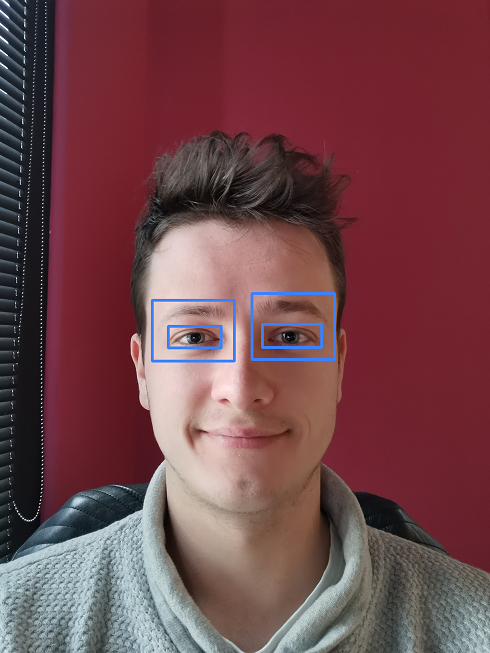
\includegraphics[scale=0.6]{img/pupil_section/expected_eyes_region.png}
        \caption{Przybliżony obszar oczu, który chcę wykrywać}
        \label{fig:expected_eyes_region}
    \end{center}
\end{figure}

\subsection{Warunki testowania}

Oba algorytmy zostaną przetestowane na wykrytych przez algorytm HOG twarzach ze zdjęć 500x500. W tym teście postanowiłem odrzucić już rozdzielczość 300x300, ze względu, że na części z nich osoba jest już bardzo oddalona, co skutkuje bardzo małym rozmiarem oczu. W przypadku korzystania z przedniej kamery telefonu nie będą występowały takie odległości między twarzą, a urządzeniem. Z tego powodu takie warunki nie przyniosłyby znaczących i wartościowych w kontekście pracy dyplomowej wyników. 
\par
Testy zostaną przeprowadzone w przestrzeni barw RGB oraz w skali szarości.

\subsection{Badanie skuteczności detekcji}

Na początku porównywana była skuteczność zaprezentowanych metod. Chociaż w pewien sposób procent detekcji był już przedstawiony podczas dostrajania algorytmów, to tutaj zostały skonfrontowane ze sobą oba algorytmy.
\par
W przypadku metody opartej o facemarki, niewykryte oczy zarówno otwarte jak i zamknięte mogą oznaczać źle określenie położenia lub złą klasyfikacje do jednej z tych grup. Przykładowo oko otwarte mające $EAR$ mniejszy niż ustalony próg klasyfikowane było jako zamknięte, co skutkowało oznaczeniem jako błędna detekcja. 

\begin{table}[!h]
\label{tab:eye_detection_accuracy_result}
\centering
\caption{Skuteczność algorytmów detekcji twarzy}
\resizebox{\textwidth}{!}{%
\begin{tabular}{|c|c|c|c|c|c|c|}
\hline
 &
  \textbf{\begin{tabular}[c]{@{}c@{}}Prawidłowe\\ detekcje\end{tabular}} &
  \textbf{\begin{tabular}[c]{@{}c@{}}Perfekcyjne\\ detekcje\end{tabular}} &
  \textbf{\begin{tabular}[c]{@{}c@{}}Częściowo\\ dobre\\ detekcje\end{tabular}} &
  \textbf{\begin{tabular}[c]{@{}c@{}}Złe\\ detekcje\end{tabular}} &
  \textbf{\begin{tabular}[c]{@{}c@{}}Niewykryte\\  oczy otwarte\end{tabular}}  &
 \textbf{\begin{tabular}[c]{@{}c@{}}Niewykryte\\  oczy zamknięte \end{tabular}} \\ \hline \hline

\textbf{Facemarki oczu RGB} &
  144 &
  142 &
  2 &
  12 &
  6 &
  6  \\ \hline
  
\textbf{\begin{tabular}[c]{@{}c@{}}Facemarki oczu \\ sk. szaro. \end{tabular}} &
  145 &
  140 &
  5 &
  11 &
  1 &
  6  \\ \hline
  
\textbf{Haar RGB} &
  133 &
  95 &
  38 &
  23 &
  9 &
  11  \\ \hline
  
\textbf{Haar sk. szaro.} &
  130 &
  95 &
  35 &
  26 &
  11 &
  7  \\ \hline
  
  \hline
\end{tabular}%
}
\end{table}

Najlepsze wyniki uzyskała metoda oparta na punktach charakterystycznych twarzy w trójkanałowej przestrzeni barw. Udało się jej wykryć średnio  $87\%$ wszystkich oczu. A w przypadku przestrzeni RGB aż $98,6\%$ z nich perfekcyjnie. Ta druga statystyka jest dużo lepsza niż w przypadku metod Haar które uzyskały raptem $57\%$. Ogólnie algorytm wykorzystujący facemarki był lepszy od drugiego o około $10\%$.
\par
Co ciekawe większą liczbę dobrych detekcji metoda oparta o facemarki uzyskała w przypadku obrazów w skali szarości, ale mniej perfekcyjnych. Natomiast, algorytm Haar lepiej poradził sobie w przypadku trójkanałowego zestawu barw, ale wykrywał ona więcej zamkniętych oczu przez co w tej statystyce wypadł gorzej niż w skali szarości. 

\vspace{5mm}

Ważną różnicą w działaniu obu algorytmów jest kształt i rozmiar oznaczanego obszaru. Metoda oparta o klasyfikatory zwraca kwadratowy region, zawierający dużo większą część twarzy niż same oczy. Natomiast facemarki tworzą obszar o kształcie prostokąta o dowolnym stosunku boków i zawierają głównie samą gałkę oczną. Zmniejsza to ilość punktów, które mogą przeszkadzać np. w detekcji źrenic.

\subsubsection{Badanie szybkości detekcji} \label{section:eye_detection_speed_img}


Dla detekcji oczu z użyciem facemarków zostały przedstawione dwa wyniki czasowe - jeden uwzględniający czas wykrycia punktów charakterystycznych, a drugi bez. Związane jest to z faktem, że mimo iż do wykorzystania tej metody niezbędna jest detekcja facemarków, to etap taki i tak będzie wykonany, ponieważ punkty te są używane np. do stwierdzenia mrugnięcia. W przypadku czasów zawierających algorytm punktów charakterystycznych test był przeprowadzony dla dwóch przestrzeni barw. Natomiast, na szybkość przekształcenia facemarków w obszar oka nie wpływa liczba kanałów, ponieważ nie operuje on na pikselach, tylko na zwróconych punktach kartezjańskich. Z tego powodu przedstawiony jest tylko jeden wynik.

\begin{table}[!h]
\label{tab:eye_detect_speed_RGB}
\centering
\caption{Czas przetwarzania algorytmów detekcji twarzy dla obrazów RGB}

\begin{tabular}{|c|c|c|c|}
\hline
 & 
  \textbf{\begin{tabular}[c]{@{}c@{}}Całkowity czas \\ przetwarzania \end{tabular}} &
  \textbf{\begin{tabular}[c]{@{}c@{}}Średni czas\\ przetwarzania \\ pojedynczej iteracji\end{tabular}} &
  \textbf{\begin{tabular}[c]{@{}c@{}}Średni czas\\przetwarzania \\ pojedynczego\\zdjęcia\end{tabular}} \\ \hline\hline
  
\textbf{\begin{tabular}[c]{@{}c@{}}Facemarki oczu RGB\\ (z detekcją facemarków)\end{tabular}} & 
  5,638 s &
  0,281 s &
  0,00361 s    \\ \hline
  
  \textbf{\begin{tabular}[c]{@{}c@{}}Facemarki oczu sk. szaro. \\ (z detekcją facemarków)\end{tabular}} & 
  5,803 s &
  0,290 s &
  0,00372 s    \\ \hline
  
\textbf{\begin{tabular}[c]{@{}c@{}}Facemarki oczu \\ (bez detekcją facemarków)\end{tabular}} & 
  0,024 s &
  0,00122 s &
  0,00000157 s  \\ \hline
  
\textbf{Haar RGB} & 
  26,219 s &
  1,310 s &
  0,0168 s     \\ \hline
  
\textbf{Haar sk. szaro.} & 
  25,830 s &
  1,291 s &
  0,0165 s    \\ \hline
  
  \hline
\end{tabular}%

\end{table}

Wyniki bezdyskusyjnie pokazują dużo większą szybkość detekcji oczu z użyciem facemarków. Nawet biorąc pod uwagę czas wykrycia punktów charakterystycznych metoda ta była ponad $4$ razy szybsza od algorytmu opartego na klasyfikatorach kaskadowych Haar. 
\par
Tworzenia obszarów z punktów charakterystycznych osiągnęło czas rzędu $10^{-5}$, co w porównaniu do pozostałych algorytmów wykorzystywanych w projekcie jest praktycznie zerowy. Tak krótki czas przetwarzania sprawia, że nie będzie on miał żadnego wpływu na ilość klatek na sekundę podczas odbierania obrazu na żywo z kamery.
\par
Przestrzeń barw nie miała znaczącego wpływu na czas detekcji, a wyniki w przypadku trójkanałowych kolorów były porównywalne do skali szarości.

\subsection{Testowanie na obrazie z kamery na żywo}

Detekcja oczu została przetestowana również na obrazie z kamery na żywo. Warunki przeprowadzenia eksperymentu zostały opisane w rozdz. \hyperref[{section:face_detection_test_live}]{\ref{section:face_detection_test_live}}.

\subsubsection{Skuteczność detekcji}

Obserwując na żywo detekcje oczu byłem w stanie wysnuć kilka wniosków na temat badanych algorytmów.

\vspace{4mm}

Przede wszystkim oba działały bardzo stabilnie. Nie występowało nieuzasadnione gubienie obszaru oczu podczas statycznego położenia głowy. 
\par
W metodzie Haar występował problem przy mocnym skręceniu głowy w bok. Zwracany był wtedy często błędny i bardzo powiększony obszar dalszego oka. 
\par
Natomiast detekcja oczu na podstawie facemarków miała problemu z mocno przymkniętymi oczami. Wskaźnik EAR sygnalizował wtedy je jako zamknięte przez co algorytm nie zwracał ich regionu.

\subsubsection{Szybkość detekcji}

Ze względu na praktycznie zerowy obciążenie podczas przekształcania facemarków w obszar twarzy (patrz rozdz. \hyperref[{section:eye_detection_speed_img}]{\ref{section:eye_detection_speed_img}}) wyniki dla facemarków zostały skopiowane z rezultatów uzyskanych przez algorytm Kazemi podczas porównania metod nakładania punktów charakterystycznych na obraz z kamery na żywo  w rozdz. \hyperref[{section:facemark_speed_live}]{\ref{section:facemark_speed_live}}.
\par
Ponownie detekcja twarzy odbywała się przy zastosowaniu algorytmu \textit{HOG} dostarczając obraz RGB.

\begin{table}[!h]
\label{tab:eye_detection_speed_live}
\centering
\caption{Szybkość algorytmów detekcji oczu dla obrazu na żywo z kamery [klatki/s]}
\begin{tabular}{|c|c|c|c|c|c|}
\hline
 \textbf{\begin{tabular}[c]{@{}c@{}}Warunki\end{tabular}} &
  \begin{tabular}[c]{@{}c@{}}1.\end{tabular} &
  \begin{tabular}[c]{@{}c@{}}2.\end{tabular} &
  \begin{tabular}[c]{@{}c@{}}3.\end{tabular} &
  \begin{tabular}[c]{@{}c@{}}4.\end{tabular} &
  \textbf{\begin{tabular}[c]{@{}c@{}}Średnia:\end{tabular}}\\ \hline \hline
\textbf{Haar RGB} &
  11,698 &
  13,600 &
  12,290 &
  12,942 &
  12,632  \\ \hline

\textbf{Haar sk. szaro.} &
  11,956 &
  12,403 &
  12,333 &
  12,472 &
  12,290 \\ \hline
  
\textbf{Znaczniki RGB} &
  15,887 &
  15,941 &
  16,077 &
  16,171 &
  16,019  \\ \hline
  
\textbf{Znaczniki sk. szaro.} &
  15,747 &
  16,146 &
  15,866 &
  16,096 &
  15,963 \\ \hline

  \hline
\end{tabular}%

\end{table}

Test ten pokazał znaczną przewagę szybkościową metody opartej na facemarkach. Klasyfikatory kaskadowe uzyskały około $23\%$ mniejszą liczbę klatek na sekundę.



\subsection{Wybór algorytmu}

Porównanie dwóch algorytmów detekcji oczu bezdyskusyjnie pokazało wyższość metody opartej na facemarkach nad klasyfikatorem kaskadowym Haar. Punkty charakterystyczne uzyskały lepszy procentowo wynik prawidłowych detekcji, a dodatkowo w teście na statycznych zdjęciach prawie wszystkie były perfekcyjne. Próby szybkościowe jednoznacznie wskazały na facemarki, które były $4$ razy szybsze od Haar, a jeśli brać pod uwagę jedynie czas tworzenia obszarów to ponad tysiąckrotnie.
\par
Na podstawie przeprowadzonych testów zostały wybrane facemarki do detekcji oczu i to ten algorytm będzie wykorzystywany w projekcie i pracy dyplomowej.